

\documentclass[runningheads,a4paper]{llncs}

\usepackage{amssymb}
\setcounter{tocdepth}{3}
\usepackage{graphicx}
\usepackage{amsmath}
%\usepackage{amsfonts}
%\usepackage{amsthm}
\usepackage{subfigure}
%\usepackage{caption} 
%\usepackage{subcaption}
%\usepackage{cite}
\usepackage{hyperref}
\usepackage{url}
\usepackage{clrscode4e}
\urlstyle{same}
\newcommand{\keywords}[1]{\par\addvspace\baselineskip
\noindent\keywordname\enspace\ignorespaces#1}

\makeatletter
\let\c@lemma=\c@theorem
\let\c@corollary=\c@theorem
\let\c@fact=\c@theorem
\makeatother

\let\realendproof=\endproof
\def\endproof{\hspace*{\fill}$\Box$\realendproof}


\begin{document}

\mainmatter  

\title{Experiments on ANTS Algorithms Without Communication}
\author{Fermi Ma \and Nicolas Rakover \and Erik Waingarten}
\institute{MIT}

\maketitle

\section{Introduction}

We study the \emph{Ants Nearby Treasure Search} (ANTS) problem for modelling collective foraging in animal groups. $k$ identical probabilistic agents search for treasure located by an adversary $D$ units away from a central location. The problem is a generalization of a previously studied problem, the \emph{cow-path} problem, which is the case where $k = 1$. 

Our project is a combination of a reading project and an experimental project. For the reading project component, we survey three known algorithms for the ANTS algorithm by Feinerman et al. and Lenzen et al. For the experimental project, we show the results of tests run on these algorithms to determine the constants in their runtimes.

The paper is organized as follows. In Section~\ref{problem statement}, we formally state and motivate the problem. We also give a simple argument for why any algorithm solving the problem takes $\Omega(D+D^2/k)$ time. We then outline different algorithm types, and give high-level overviews of the spiral, harmonic, and lines algorithms. In Section~\ref{spiral}, we give a more in-depth explanation of the details of the spiral algorithm of Feinerman et al. We do this for the harmonic algorithm in Section~\ref{harmonic}, and for the lines algorithm in Section~\ref{lines}. In Section~\ref{experiments}, we shift our focus to the experimental part of our project. In that section, we describe our hypotheses, our experimental setup, the results, and our interpretation of the results. We give concluding remarks in Section~\ref{conclusion}. 

\section{Problem Setup and Basics}
\label{problem statement}

There are $k$ mobile agents searching for treasure in the two-dimensional grid $G$ with vertex set $\mathbb{Z}^2$. All $k$ agents start the search from a central \emph{source} node $s \in G$. An adversary places the treasure at some target node $\tau \in G$ at a \emph{hop distance} $D$ away from $s$. The hop distance is the minimum number of grid edges that must be traversed to get from one node to another, and is also known as the taxicab distance. We denote the hop distance from the starting node $s$ to some point $t$ as $d(t)$. The goal of the agents is for one of them to find the treasure by reaching the node $\tau$.

It is assumed that the agents act synchronously, and that they all start their search at the same time $t_0$. Each edge traversal costs one unit of time, so the total time (or cost) it takes to run an algorithm is the number of edges traversed by the first agent to find the treasure. The cost of a given algorithm $\mathcal{A}$ is the expected time it takes to find the treasure, which is denoted by $T_\mathcal{A}(D,k)$.

\subsection{A Simple Lower Bound}

There is a simple $\Omega(D+D^2/k)$ lower bound which follows from the following argument. The time it takes $T$ for an algorithm to run must satisfy $T \geq D$, or else it is not even possible to reach treasure $D$ units away. 

Also, $T$ must satisfy $T \geq D^2/4k$. To see why, suppose not. Then $T < D^2/4k$, and in particular $2kT < D^2/2$. Thus, out of all the points that are at most $D$ away from the source $s$, by time $2T$, strictly less than half of them have been visited. This implies that some node at most $D$ units away is visited with probability less than $1/2$ by time $2T$. If the adversary simply places the target at that node, then the expected time to find the treasure is strictly greater than $T$, which is a contradiction.

Note this lower bound holds even if the agents knows the total number of agents. 

\subsection{Types of Algorithms}
We will focus on three kinds of algorithms:
\begin{itemize}
\item Spiral algorithms
\item Lines algorithms
\item Harmonic search algorithm
\end{itemize}

And each algorithm has two flavours: \emph{uniform} and \emph{non-uniform}. We say that an algorithm is non-uniform in parameter $p$ if $p$ is an input to the algorithm. If the parameter $p$ is not an input, then the algorithm is uniform in $p$. 

For example, a spiral algorithm which is non-uniform in $k$ is the algorithm where agents can know how many total agents there are. An algorithm which is non-uniform in $D$ has an upper bound on the hop distance of the treasure. 

The spiral and Harmonic search algorithms are similar strategies and were introduced by \cite{feinerman2012collaborative}. Both rely on the ``spiral" procedure, in which an agent covers a space of $\sqrt{d}$ grid cells in $O(d)$ time. Figure~\ref{fig:spiral} shows a possible spiral routine.
There will be two kinds of spiral algorithms, non-uniform in $k$ and uniform in $k$. There will be three kinds of lines algorithms, non-uniform in $D$, non-uniform in $k$, and uniform in both $k$ and $D$. The Harmonic search algorithm is extremely simple and uniform in both $k$ and $D$. 

\begin{figure}
\centering
\label{fig:spiral}
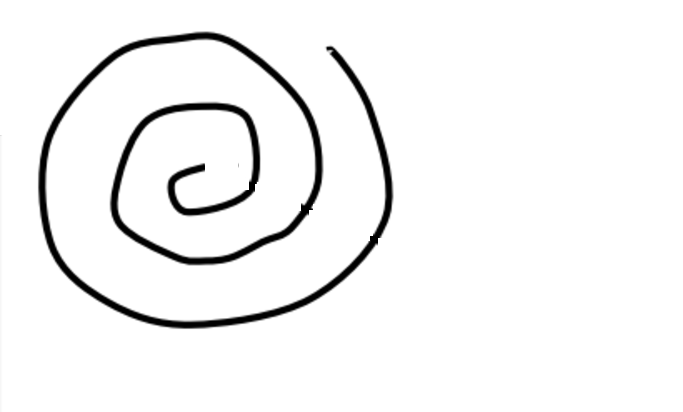
\includegraphics[width=0.4\linewidth]{justspiral.pdf}
\caption{Possible spiral, covering $\sqrt{d}$ grid cells in $O(d)$ time}
\end{figure}

\section{Spiral Algorithms}
\label{spiral}

The following short explanations are from \cite{feinerman2012collaborative}.

\subsubsection{Non-uniform in $k$}

Given the number of agents taking part in the search, we could imagine an algorithm in which the grid in divided into $k$ parts, similar to a pizza being divided into $k$ equal parts. Each agent could cover his portion, and this would yield an asymptotically optimal algorithm. However, this assumes that the agents can communicate with each other and decide which portion belongs to which agent. 

In order to get around this, we can introduce some randomization. If each agent picks a random grid cell within some distance $D$, travels to that distance and performs a spiral of sufficiently large size, it can expect that all agents together will search new areas. If we repeat this sufficiently many times, we can expect that the whole area within distance $D$ was covered. Then we just need to estimate the value of $D$.

This is what the spiral algorithms does when its non-uniform in $k$. 

\begin{codebox}
\Procname{Each agent performs the following double loop}
\li \For $j$ from $1$ to $\infty$, \Then
\li \For $i$ from $1$ to $j$ \Then
\li Go to a node chosen uniformly at random from nodes a distance $2^{i}$
\li Perform a spiral search for $2^{2i+2}/k$ steps
\li Return to source \End \End 
\end{codebox}

We provide a sketch of the proof to show the algorithm has expected running time $O(D + D^2/k)$. Note that the time until agents reach some value of $j$ is $O(2^j + 2^{2j}/k)$. Also, note that once $i \geq \log D$, the spiral will intersect the ball of radius $D$ significantly, and so the probability that an agent finds the treasure is some constant $\beta$. Therefore, the probability that no agents find it after $l$ phases of $i$ is $(1 - \beta/k)^{kl}$, which is also at most some constant probability $\gamma$.

So for each additional $l$ values of $j$ once $j = \lceil \log D \rceil$, there are $l^2/2$ phases where $i \geq \log D$, and so the probability that a round takes $O(2^{j + l} + 2^{2(j+l)}/k)$ is $\gamma^{l^2/2}$, and so in the computation of the expected value, the sum of all $l$ converges to some constant. And we are left with a runtim of $O(2^{j} + 2^{2j}/k)$ for $j = \log D$. This finishes the sketch.

\subsubsection{Uniform in $k$}

Once we have the spiral algorithm non-uniform in $k$, we can make it uniform in $k$ by successively doubling estimates of $k$. This means that at each stage, we take a guess of what $k$ is, and we simulate the algorithm. There is some additional bookkeeping to ensure that enough iterations are made, but the optimization is similar. There is higher lower bound on how fast these algorithms can run, and we get a multiplicative factor of $f(\log k)$, where $f$ is a function such that $\sum \dfrac{1}{f(n)}$ converges. There is a corresponding lower bound that shows this algorithm is asymptotically optimal.

\section{Harmonic Algorithm}
\label{harmonic}

\section{Lines Algorithm}
\label{lines}

The lines algorithm is the study of \cite{lenzen2014trade}, where they cover a lines algorithm which is non-uniform in $D$ and non-uniform in $k$. We use the ideas of \cite{feinerman2012collaborative} to design a lines algorithm which is uniform in both $k$ and $D$. The lines algorithm has many optimizations since \cite{lenzen2014trade} are trying to reduce \emph{selection complexity}. Selection complexity is a metric which measures how likely an algorithm is to occur naturally in nature. Of course, this notion is very vague, but formally, the selection complexity $\chi$ of an algorithm $A$ is $\chi(A) = b + \log l$ where $b$ is the amount of memory usage and $l$ is smallest $l$ for which the algorithm does not need finer probabilities than $2^{-l}$. In \cite{lenzen2014trade}, Lenzen et al. provided a lines algorithm with selection complexity $O(\log \log D)$.

\subsubsection{Non-uniform in $D$} First, we will explain the simple lines algorithm which is non-uniform in $D$. Remember, $D$ is an upper bound on the distance the treasure. The lines algorithm is very simple to explain. With probability $\frac{1}{2}$, an agent moves up, otherwise, it moves down. Then it continues moving in that direction until a coin with head probability $\frac{D-1}{D}$ lands on tails. It repeats the process for the left and right directions. The pseudocode is shown, $C_p$ will denote a coin which lands heads with probability $p$, and so $C_p$ will return a 0 or 1, with 0 denoting heads.

The algorithm relies on it novel way of walking in lines by approximately counting. The following procedure shows how an agent would move in a particular direction. 

\begin{codebox}
\Procname{moveDirection(dir)}
\li \While $C_{\frac{D-1}{D}} = 0$ \Then
\li agent moves in direction dir \End
\end{codebox}

Note that the above algorithm, while it uses contant memory, it does need to sample from a distribution with probability as fine as $\frac{1}{D}$. This is fine, since in this case, $l = \log D$. 
Now that we know how agents move in a particular direction, they randomly pick a direction to travel.

\begin{codebox}
\Procname{Each agent performs the following iteration}
\li dir[0] $\leftarrow$ up, dir[1] $\leftarrow$ down
\li $i \leftarrow C_{\frac{1}{2}}$
\li moveDirection($i$)
\li \If $C_{\frac{1}{2}} = 0$ \Then
\li moveDirection(left)
\li \Else moveDirection(right) \End \End
\li return to origin
\end{codebox}

The one thing to note is that the last line, ``return to origin" would need to keep the location of the ant. This would require $\log D$ memory, which we cannot afford; however, it is an assumption in the model that agents can return to the origin.

% TO DO
The sketch of the proof of correctness is the following ...????

\subsubsection{Uniform in $D$}

\section{Experiments and Results}
\label{experiments}

\subsection{Hypotheses}

\subsection{Experimental Setup}

\subsection{Findings}

\subsection{Interpretation}

\section{Conclusion}
\label{conclusion}

\bibliographystyle{plain}
\bibliography{references}

\end{document}
